\documentclass[a4paper, 10pt]{article}
\usepackage[T1]{fontenc}
\usepackage[utf8]{inputenc}
\usepackage[slovene]{babel}
\usepackage{csquotes}
\usepackage{lmodern}
\usepackage{amsmath}
\usepackage{leftidx}
%\usepackage[backend=biber, style=numeric]{biblatex}
\usepackage{amssymb}
\usepackage{amsthm}
\usepackage{amsfonts}
\usepackage{graphicx, float}
\usepackage{amsthm}
\usepackage{mathrsfs}
\usepackage{mathtools}
\usepackage{url}
\usepackage{subfigure}
\usepackage{multirow}
\usepackage{lipsum}
\usepackage{wrapfig}
\usepackage{tikz}
\usepackage[format=plain, font=small, labelfont=bf, textfont=it, justification=centerlast]{caption}
\usepackage{booktabs}
\usepackage{siunitx}
\usepackage{ulem}
\usepackage{cancel}
\usepackage{algorithm2e}
\usepackage{color, listings}
%\usepackage{cleveref}

\newtheorem{izr}{Izrek}
\newtheorem{lem}{Lema}
\newtheorem{trd}{Trditev}
\newtheorem{posl}{Posledica}[izr]

\newcounter{defcount}
\newcounter{opombe}
\newcounter{primercount}
\newcounter{zgledcount}

\newenvironment{opomba}{\begin{flushleft}\refstepcounter{opombe}\textbf{Opomba \arabic{opombe}:}}{\hfill\end{flushleft}}
\setlength{\parindent}{0mm}

\newenvironment{primer}{\begin{flushleft}\refstepcounter{primercount}\textbf{Primer \arabic{primercount}:}}{\hfill\end{flushleft}}
\setlength{\parindent}{0mm}

\newenvironment{zgled}{\begin{flushleft}\refstepcounter{zgledcount}\textbf{Zgled \arabic{zgledcount}:}}{\hfill\end{flushleft}}
\setlength{\parindent}{0mm}

\newenvironment{definicija}{\begin{flushleft}\refstepcounter{defcount}\textbf{Definicija \arabic{defcount}:}}{\hfill\end{flushleft}}
\setlength{\parindent}{0mm}

\newenvironment{resitev}{\begin{flushleft}\textit{Rešitev:}}{\hfill\end{flushleft}}
\setlength{\parindent}{0mm}

\definecolor{gray}{rgb}{0.5, 0.5, 0.5}
\definecolor{mauve}{rgb}{0.58, 0.82, 0}
\definecolor{dkgreen}{rgb}{0, 0.6, 0}
\lstset{frame=tb,
	language=Matlab,
	aboveskip=3mm,
	belowskip=3mm,
	showstringspaces=false,
	columns=flexible,
	basicstyle={\small\ttfamily},
	numbers=none,
	numberstyle=\tiny\color{gray},
	keywordstyle=\color{blue},
	commentstyle=\color{dkgreen},
	stringstyle=\color{mauve},
	breaklines=true,
	breakatwhitespace=true,
	tabsize=3}

\newcommand{\naslov}[1]{\textit{#1}}
\newcommand{\abs}[1]{\ensuremath{\lvert #1 \rvert}}
\newcommand{\mth}[1]{\ensuremath{\mathbb{#1}}}
\newcommand{\R}{\mth{R}}
\newcommand{\Z}{\mth{Z}}
\newcommand{\Zp}{\mth{Z}^{+}}
\newcommand{\N}{\mth{N}}
\newcommand{\No}{\mth{N}_0}
\newcommand{\C}{\mth{C}}
\newcommand{\Q}{\mth{Q}}
\newcommand{\Qu}{\mth{Q}_u}
\newcommand{\pojem}[1]{\emph{#1}}
\newcommand{\con}{\ensuremath{\mathscr{C}}}
\newcommand{\padex}[2]{\ensuremath{{#1}^{\underline{#2}}}}
\newcommand{\rastx}[2]{\ensuremath{{#1}^{\bar{#2}}}}
\newcommand{\map}[3]{\ensuremath{{#1}: {#2} \rightarrow {#3}}}
\newcommand{\pra}[3]{{#1}{\ast}({#2}) = {#3}}

\title{Numerično reševanje sistemov diferencialnih enačb \\ {\large Projektna naloga pri predmetu Diferencialne enačbe}}
\date{2.~6.~2024}
\author{Jimmy Zakeršnik}
%===============================================================================
\begin{document}
	\maketitle
	\thispagestyle{empty}
	\newpage
	\tableofcontents
	\newpage
	\section{Uvod}
	Tekom študija diferencialnih enačb lahko hitro naletimo na posebne primere, katerih splošne rešitve bodisi ne znamo izraziti eksplicitno, bodisi te rešitve sploh ne znamo poračunati (morda z izjemo nekaterih posebnih primerov). V nekaterih od teh primerov lahko posežemo po raznih metodah, ki nam dajo neko partikularno rešitev, v nekaterih pa tudi to (s trenutnimi metodami) ni možno. V slednji situaciji pridejo prav numerične metode za reševanje diferencialnih enačb, ki se neznani analitični rešitvi vsaj približajo. Seveda imajo nekatere metode višji red konvergence in v danem času ali danem številu korakov vrnejo rezultat, ki je boljši približek dejanske rešitve, kot pa druge. V tej nalogi bomo obravnavali Eulerjevo metodo in metodo Runge-Kutta reda $4$, ki se uporabljajo za reševanje sistemov diferencialnih enačb. Dodatno bomo pokazali, kako lahko s tema metodama rešujemo diferencialne enačbe višjih redov, preko pretvorbe v sistem diferencialnih enačb. Informacije bomo primarno črpali iz vira \cite{bib:Matlab}. Na koncu bomo omenjeni metodi primerjali na podlagi grafov rešitev.
%%%%%%%%%%%%%%%%%%%%%%%%%%%%%%%%%%%%%%%%%%%%%%%%%%%%%%%%%%%%%%%%%%%%%%%%%%%%%%%%%%%%%%	
	\section{Eulerjeva metoda}
		V tem poglavju bomo na kratko opisali Eulerjevo metodo za reševanje sistemov diferencialnih enačb (krajše: SDE). Za lažjo predstavo bomo to najprej storili na primeru sistema \begin{align*}
			\dot{x}(t) &= f(t, x, y, z) \\
			\dot{y}(t) &= g(t, x, y, z) \\
			\dot{z}(t) &= h(t, x, y, z)
		\end{align*} z začetnimi pogoji $x(t_0) = x_0, y(t_0) = y_0$ in $z(t_0) = z_0$.
		
		Pod predpostavko, da so funkcije $f, g$ in $h$ vse $\mathcal{C}^1$ funkcije na neki okolici $D$ točke $t_0$, lahko za funkcije $x(t), y(t)$ in $z(t)$ preko uporabe Lagrangeevega izreka izpeljemo Eulerjevo metodo: \begin{align*}
			x(t) - x(t^\circ) &= \dot{x}(t^*)(t - t^\circ) = f(t^*, x^*, y^*, z^*)(t - t^\circ) \\
			y(t) - y(t^\circ) &= \dot{y}(t')(t - t^\circ) = g(t', x', y', z')(t - t^\circ) \\
			z(t) - z(t^\circ) &= \dot{z}(t")(t - t^\circ) = h(t", x", y", z")(t - t^\circ)
		\end{align*} za poljubna $t, t^\circ \in D$ in neke $t^*, t'$ in $t"$, ki se nahajajo na neki daljici med $t$ in $t^\circ$.
		Denimo, da iščemo rešitev sistema na intervalu $[t_0, b]$, na katerem so $f, g$ in $h$ $\mathcal{C}^1$. Ta interval ekvidistančno razdelimo na $n$ podintervalov: \begin{align*}
			d &= \frac{b - t_0}{n} \\
			t_{k+1} &= t_k + d ~\forall k\in \{0, 1, \ldots, n-1\}
		\end{align*} 
		Dodatno, za $\forall k\in \{0, 1, \ldots, n-1\}$ določimo $x_{k+1}, y_{k+1}$ in $z_{k+1}$ na naslednji način: \begin{align*}
			x_{k+1} &= x_k + df(t_k, x_k, y_k, z_k) \\
			y_{k+1} &= y_k + dg(t_k, x_k, y_k, z_k) \\
			z_{k+1} &= z_k + dh(t_k, x_k, y_k, z_k) \\
		\end{align*}
		
		Recept za reševanje poljubnega SDE oblike $\dot{x}_i(t) = f_i(t, x_1(t), \ldots, x_n(t))~ \forall i \in \{1, 2, \ldots, n\}$, z začetnim pogojem $[x_1(t_0), \ldots, x_n(t_0)] = [x^{(0)}_1, \ldots, x^{(0)}_n]$, s pomočjo Eulerjeve metode, se torej da povzeti na naslednji način: ">V vsakem koraku istočasno uporabimo Eulerjevo metodo na vsaki funkciji $x_i$"<. 
		
		Preden navedemo algoritem v Matlabu, si oglejmo še primer uporabe.
		\begin{primer}
			\label{prim:Euler1}
			Za SDE \begin{align*}
				\dot{x} &= 2x + 3y + z\\
				\dot{y} &= 2x + y - 3z \\
				\dot{z} &= x + 2y + 3z
			\end{align*} na območju $[0, 1]$, pri začetnem pogoju $[x(0), y(0), z(0)] = [-2'7, 2'8, 2'1]$ (tukaj za preglednost namesto decimalne vejice uporabljamo simbol ') izvedi dva koraka Eulerjeve metoda za $d = 0'05$.
		\end{primer}
		
		\begin{resitev}
			Najprej si izpišimo naše $f, g$ in $h$: \begin{align*}
				f(t, x, y, z) &= 2x + 3y + z\\
				g(t, x, y, z) &= 2x + y - 3z\\
				h(t, x, y, z) &= x + 2y + 3z
			\end{align*}
			
			Sedaj določimo $t_1, x_1, y_1$ in $z_1$: \begin{align*}
				t_1 &= t_0 + d = 0 + 0'05 = 0'05 \\
				x_1 &= x_0 + df(t_0, x_0, y_0, z_0) = -2'7 + 0'05(2(-2'7) + 3(2'8) + (2'1)) \\
				y_1 &= y_0 + dg(t_0, x_0, y_0, z_0) = 2'8 + 0'05(2(-2'7) + (2'8) - 3(2'1))\\
				z_1 &= z_0 + dh(t_0, x_0, y_0, z_0) = 2'1 + 0'05((-2'7) + 2(2'8) + 3(2'1))
			\end{align*}
			Ko to poračunamo, dobimo: \begin{align*}
				t_1 &= 0'05 \\
				x_1 &= -2'445 \\
				y_1 &= 2'355 \\
				z_1 &= 2'56 
			\end{align*}
			
			Sedaj s pomočjo teh vrednosti določimo $t_2, x_2, y_2$ in $z_2$:
			\begin{align*}
				t_2 &= t_1 + d = 0'05 + 0'05 = 0'1 \\
				x_2 &= x_1 + df(t_1, x_1, y_1, z_1) = -2'445 + 0'05(2(-2'445) + 3(2'355) + (2'56)) \\
				y_2 &= y_1 + dg(t_1, x_1, y_1, z_1) = 2'355 + 0'05(2(-2'445) + (2'355) - 3(2'56)) \\
				z_2 &= z_1 + dh(t_1, x_1, y_1, z_1) = 2'56 + 0'05((-2'445) + 2(2'355) + 3(2'56))
			\end{align*}
			
			Tako dobimo (z zaokrožitvijo na tri decimalke):
			\begin{align*}
				t_2 &= 0'1 \\
				x_2 &= -2'208 \\
				y_2 &= 1'844 \\
				z_2 &= 3'057 \\
			\end{align*}
		\end{resitev}
		Zgornja naloga je tudi primer SDE, v katerem bi težko določili analitično rešitev. V resnici gre za sistem LDE, katerega karakteristični polinom se glasi $-x^3 + 6x^2 - 10x - 6$. Ničle tega polinoma je težko določiti s standardnimi metodami, kar pomeni, da je tudi težko določiti Jordanovo formo za matriko sistema in posledično je težko določiti splošno analitično rešitev.
		
		Oglejmo si sedaj algoritem za Eulerjevo metodo za SDE v matlabu:
		
		\begin{lstlisting}
			function [T, Z] = SDEeuler(F, a, b, Za, k)
			% Vhodni podatki:
			% F je SDE, zapisan kot niz 'F'
			% a in b sta krajisci intervala
			% Za = [x1(a), ..., xn(a)] zacetni pogoji
			% k je stevilo korakov metode
			% Izhodni podatki:
			% T vektor, ki vsebuje tk - vektor korakov
			% Z matrika, v kateri je na koordinati (i, j) priblizek vrednosti funkcije xj v tocki t(i+1)
			h = (b-a)/k; % Dolocimo velikost koraka
			n = length(Za); % Stevilo funkcij oz. enacb v sistemu
			T = zeros(1, k+1); % Pripravimo vektor za korake
			Z = zeros(k+1, n); % Pripravimo matriko Z
			T=a:h:b; % a:h:b: je seznam stevil od a do b, s korakom h
			Z(1, :) = Za; % Prvo vrstico matrike Z napolnimo z zacetnimi pogoji
			
			for j = 1:k
				Z(j+1, :) = Z(j, :) + h*feval(F, T(j), Z(j, :)); % Poracunamo (j+1)-to vrstico matrike Z
			end
		\end{lstlisting}
		
		Zgornja koda je zapisana v Matlab skripti \emph{SDEeuler.m}, v skripti \emph{Resitve1DE.m} pa se nahaja rešitev SDE iz primera \ref{prim:Euler1} pri $20$ korakih tako z Eulerjevo metodo kot tudi z metodo Runge-Kutta reda $4$. Hitro se da premisliti, da ima metoda red konvergence $1$, saj gre v bistvu za večkratno uporabo navadne Eulerjeve metode, ki je reda $1$.
		
		Sedaj si poglejmo še, kako bi lahko s to metodo rešili diferencialno enačbo višjega reda.
		
		Denimo, da imamo pred seboj Cauchyjevo nalogo podano z DE reda $n$ $$x^{(n)}(t) = F(t, x(t), \dot{x}(t), \ldots, x^{(n-1)}(t))$$ ter z začetnimi pogoji $$[x(t_0), \dot{x}(t_0), \ldots, x^{(n-1)}(t_0)]= [x_0, x^{(1)}_0, \ldots, x^{(n-1)}_0]$$
		
		Po znanem rezultatu iz študija diferencialnih enačb vemo, da lahko to nalogo prevedemo na SDE: \begin{align*}
			x(t) &= x_1(t) \\
			\dot{x}(t) &= x_2(t) \\
			x^{(2)}(t) &= x_3(t) \\
			&\vdots \\
			x^{(n-1)}(t) &= x_n(t) \\
			x^{(n)}(t) &= F(t, x_1, x_2, \ldots, x_n)
		\end{align*} z začetnimi pogoji $$[x_1(t_0), x_2(t_0), \ldots, x_{n}(t_0)]= [x_0, x^{(1)}_0, \ldots, x^{(n-1)}_0]$$
		Če to storimo za dano DE reda $n$, potem lahko na dobljenem SDE uporabimo metode za reševanje SDE in tako dobimo rešitev, iz katere lahko razberemo rešitev začetnega problema. Ker se v praksi najpogosteje pojavljajo DE reda $2$ (spomnimo se na primer na enačbo $mx''(t) + cx'(t) + kx(t) = g(t)$, ki opisuje gibanje vzmeti s koeficientom $k$, ko jo premaknemo iz ravnovesne lege), bomo, za demonstracijo metode, rešili enačbo reda $2$.
		
		\begin{primer}
			\label{prim:Euler2}
			Diferencialno enačbo $x''(t) + x(t) = 6\cos(t)$ z začetnima pogojema $x(0) = 2$ in $x'(0) = 3$ pretvori v SDE in na tem izvedi dva koraka Eulerjeve metode za $d = 0'05$.
		\end{primer}
		\begin{resitev}
			Najprej določimo funkcijo $F$: $F(t, x(t), x'(t)) = 6\cos(t) - x(t)$. Sedaj uvedemo $x'(t) = y(t)$ in tako dobimo SDE: \begin{align*}
				x'(t) &= y(t) \\
				y'(t) &= 6\cos(t) - x(t)
			\end{align*} z začetnimi pogoji $x(0) = x_0 = 2$ in $y(0) = y_0 = 3$. Izvedemo prvi korak metode: \begin{align*}
			t_1 &= \underline{0'05} \\
			x_1 &= x_0 + 0'05y_0 = 2 + 0'15 = \underline{2'15} \\
			y_1 &= y_0 + 0'05(6\cos(t_0) - x_0) = 3 + 0'2 = \underline{3'2}
			\end{align*}
			Nato pa še drugi korak metode: \begin{align*}
				t_2 &= \underline{0'1} \\
				x_2 &= x_1 + 0'05y_1 = 2'15 + (0'05)(3'2) = \underline{2'31}\\
				y_2 &= y_1 + 0'05(6\cos(t_1) - x_1) = 3'2 + (0'05)(6(0'999) -2'15) = \underline{3'392}
			\end{align*}
			
		\end{resitev}
		
		V Matlab skripti \emph{Resitve2DE.m} se nahaja rešitev SDE iz tega primera z Eulerjevo metodo ter z metodo Runge-Kutta reda $4$ oboje pri $20$ korakih. Več o slednji metodi bomo povedali v naslednjem poglavju.
%%%%%%%%%%%%%%%%%%%%%%%%%%%%%%%%%%%%%%%%%%%%%%%%%%%%%%%%%%%%%%%%%%%%%%%%%%%%%%%%%%%%%%		
		\section{Metoda Runge-Kutta reda $4$}
			V tem poglavju bomo opisali Runge-Kutta metodo reda $4$ za SDE in tudi navedli algoritem v Matlabu. Kot v prejšnjem poglavju, bomo tudi v tem metodo najprej opisali za primer sistema s tremi enačbami, nato pa bomo z njo rešili SDE iz primerov \ref{prim:Euler1} in \ref{prim:Euler2}.
			
			Denimo torej, da rešujemo sistem \begin{align*}
				\dot{x}(t) &= f(t, x, y, z) \\
				\dot{y}(t) &= g(t, x, y, z) \\
				\dot{z}(t) &= h(t, x, y, z)
			\end{align*} z začetnimi pogoji $x(t_0) = x_0, y(t_0) = y_0$ in $z(t_0) = z_0$.
			
			Enako kot pri Eulerjevi metodi, bomo tudi tukaj metodo na sistemu izvedli tako, da jo istočasno izvedemo na vsaki enačbi posebej. Naš interval $[a, b]$, na katerem rešujemo sistem, razdelimo na ekvidistančne točke z vmesno razdaljo $d$, enako kot pri Eulerjevi metodi. En korak metode Runge-Kutta reda $4$ za SDE, z velikostjo koraka $d$, bo torej izgledal takole: \begin{align*}
				f_1 &= f(t_k, x_k, y_k, z_k), \\
				g_1 &= g(t_k, x_k, y_k, z_k), \\
				h_1 &= h(t_k, x_k, y_k, z_k),
			\end{align*}
			\begin{align*}
				f_2 &= f(t_k + \frac{d}{2}, x_k + \frac{d}{2}f_1, y_k+ \frac{d}{2}g_1, z_k+ \frac{d}{2}h_1), \\
				g_2 &= g(t_k + \frac{d}{2}, x_k + \frac{d}{2}f_1, y_k+ \frac{d}{2}g_1, z_k+ \frac{d}{2}h_1), \\
				h_2 &= h(t_k + \frac{d}{2}, x_k + \frac{d}{2}f_1, y_k+ \frac{d}{2}g_1, z_k+ \frac{d}{2}h_1),
			\end{align*} 
			\begin{align*}
				f_3 &= f(t_k + \frac{d}{2}, x_k + \frac{d}{2}f_2, y_k+ \frac{d}{2}g_2, z_k+ \frac{d}{2}h_2), \\
				g_3 &= g(t_k + \frac{d}{2}, x_k + \frac{d}{2}f_2, y_k+ \frac{d}{2}g_2, z_k+ \frac{d}{2}h_2), \\
				h_3 &= h(t_k + \frac{d}{2}, x_k + \frac{d}{2}f_2, y_k+ \frac{d}{2}g_2, z_k+ \frac{d}{2}h_2), 
			\end{align*}
			\begin{align*} 
				f_4 &= f(t_k + d, x_k + df_3, y_k+ dg_3, z_k+ dh_3), \\
				g_4 &= g(t_k + d, x_k + df_3, y_k+ dg_3, z_k+ dh_3), \\
				h_4 &= h(t_k + d, x_k + df_3, y_k+ dg_3, z_k+ dh_3)
			\end{align*}
			
			In na koncu še \begin{align*}
				t_{k+1} &= t_k + d \\
				x_{k+1} &= x_k + \frac{d}{6}(f_1 + 2f_2 + 2f_3 + f_4) \\
				y_{k+1} &= y_k + \frac{d}{6}(g_1 + 2g_2 + 2g_3 + g_4) \\
				z_{k+1} &= z_k + \frac{d}{6}(h_1 + 2h_2 + 2h_3 + h_4)
			\end{align*}
			
			Zaradi količine računanja pri tej metodi, se bomo v primerih omejili na izvedbo enega koraka metode. Poglejmo si najprej SDE iz primera \ref{prim:Euler1}.
			
			\begin{primer}
				\label{prim:RK1}
				Za SDE \begin{align*}
					\dot{x} &= 2x + 3y + z\\
					\dot{y} &= 2x + y - 3z \\
					\dot{z} &= x + 2y + 3z
				\end{align*} na območju $[0, 1]$, pri začetnem pogoju $[x(0), y(0), z(0)] = [-2'7, 2'8, 2'1]$ (za preglednost namesto decimalne vejice uporabljamo simbol ') izvedi en korak metode Runge-Kutta reda $4$ za $d = 0'05$.
			\end{primer}
			\begin{resitev}
				Označimo funkcije $f, g$ in $h$:
				\begin{align*}
					f(t, x, y, z) &= 2x + 3y + z \\
					g(t, x, y, z) &= 2x + y - 3z \\
					h(t, x, y, z) &= x + 2y + 3z
				\end{align*}
				
				Najprej poračunamo koeficiente $f_1, g_1$ in $h_1$. \begin{align*}
					f_1 &= 2x_0 + 3y_0 + z_0 = 2(-2'7) + 3(2'8) + (2'1) = \underline{5'1}\\
					g_1 &= 2x_0 + y_0 - 3z_0 = 2(-2'7) + (2'8) - 3(2'1) = \underline{-8'9}\\
					h_1 &= x_0 + 2y_0 + 3z_0 = (-2'7) + 2(2'8) + 3(2'1) = \underline{9'2}
				\end{align*}
				Sedaj s pomočjo računalnika poračunamo še ostale koeficiente:
				\begin{align*} 
					f_2 &= 2(x_0 + \frac{d}{2}f_1) + 3(y_0 + \frac{d}{2}g_1) + (z_0 + \frac{d}{2}h_1)=\underline{4'918}\\
					g_2 &= 2(x_0 + \frac{d}{2}f_1) + (y_0 + \frac{d}{2}g_1) - 3(z_0 + \frac{d}{2}h_1)=\underline{-9'558}\\
					h_2 &= (x_0 + \frac{d}{2}f_1) + 2(y_0 + \frac{d}{2}g_1) + 3(z_0 + \frac{d}{2}h_1)=\underline{9'573}
				\end{align*} 
				\begin{align*}
					f_3 &= 2(x_0 + \frac{d}{2}f_2) + 3(y_0 + \frac{d}{2}g_2) + (z_0 + \frac{d}{2}h_2)=\underline{4'868}\\
					g_3 &= 2(x_0 + \frac{d}{2}f_2) + (y_0 + \frac{d}{2}g_2) - 3(z_0 + \frac{d}{2}h_2)=\underline{-9'611}\\
					h_3 &= (x_0 + \frac{d}{2}f_2) + 2(y_0 + \frac{d}{2}g_2) + 3(z_0 + \frac{d}{2}h_2)=\underline{9'563}
				\end{align*}
				\begin{align*} 
					f_4 &= 2(x_0 + df_3) + 3(y_0 + dg_3) + (z_0 + dh_3)=\underline{4'623}\\
					g_4 &= 2(x_0 + df_3) + (y_0 + dg_3) - 3(z_0 + dh_3)=\underline{-10'328}\\
					h_4 &= (x_0 + df_3) + 2(y_0 + dg_3) + 3(z_0 + dh_3)=\underline{9'917} 
				\end{align*}
				Na koncu določimo $t_1, x_1, y_1$ in $z_1$: \begin{align*}
					t_1 &= t_0 + d = 0 + 0'05 = \underline{0'05} \\
					x_1 &= x_0 + \frac{d}{6}(f_1 + 2f_2 + 2f_3 + f4)= \underline{-2'456}\\
					y_1 &= y_0 + \frac{d}{6}(g_1 + 2g_2 + 2g_3 + g4)= \underline{2'320} \\
					z_1 &= z_0 + \frac{d}{6}(h_1 + 2h_2 + 2h_3 + h4)= \underline{2'578}
				\end{align*}
			\end{resitev}
			
			Oglejmo si, kako bi metodo Runge-Kutta reda $4$ za SDE zapisali v Matlabu.
			\begin{lstlisting}
				function [T, Z] = SDErk4(F, a, b, Za, k)
				% Vhodni podatki:
				% F je SDE, zapisan kot niz 'F'
				% a in b sta krajisci intervala
				% Za = [x1(a), ..., xn(a)] zacetni pogoji
				% k je stevilo korakov metode
				% Izhodni podatki:
				% T vektor, ki vsebuje tk - vektor korakov
				% Z matrika, v kateri je na koordinati (i, j) priblizek vrednosti funkcije xj v tocki t(i+1)
				h = (b-a)/k; % Dolocimo velikost koraka
				n = length(Za); % Stevilo funkcij oz. enacb v sistemu
				T = zeros(1, k+1); % Pripravimo vektor za korake
				Z = zeros(k+1, n); % Pripravimo matriko Z
				T=a:h:b; % a:h:b: je seznam stevil od a do b, s korakom h
				Z(1, :) = Za; % Prvo vrstico matrike Z napolnimo z zacetnimi pogoji
				
				for j = 1:k
				k1 = h*feval(F, T(j), Z(j, :)); % Vektor koeficientov, ki jih dobimo v tocki (T(j), Z(j, :))
				k2 = h*feval(F, T(j)+h/2, Z(j, :)+k1/2); % Vektor koeficientov, ki jih dobimo v tocki (T(j)+h/2, Z(j, :)+k1/2)
				k3 = h*feval(F, T(j)+h/2, Z(j, :)+k2/2); % Vektor koeficientov, ki jih dobimo v tocki (T(j)+h/2, Z(j, :)+k2/2)
				k4 = h*feval(F, T(j)+h, Z(j, :)+k3); % Vektor koeficientov, ki jih dobimo v tocki (T(j)+h, Z(j, :)+k3)
				Z(j+1, :) = Z(j, :) + (k1 + 2*k2 + 2*k3 + k4)/6; % Poracunamo (j+1)-to vrstico matrike Z
				end
			\end{lstlisting}
			Tudi tukaj lahko hitro vidimo, da ima metoda Runge-Kutta reda $4$ za sisteme red konvergence $4$, saj gre za večkratno istočasno uporabo navadne metode Runge-Kutta reda $4$. Oglejmo si še, kako rešimo diferencialno enačbo višjega reda s pomočjo metode Runge-Kutta reda $4$ za sisteme.
			\begin{primer}
				\label{prim:RK2}
				Diferencialno enačbo $x''(t) + x(t) = 6\cos(t)$ z začetnima pogojema $x(0) = 2$ in $x'(0) = 3$ pretvori v SDE in na tem izvedi en korak metode Runge-Kutta reda $4$ za $d = 0'05$.
			\end{primer}
			\begin{resitev}
				Označimo funkciji $f$ in $g$:
				\begin{align*}
					f(t, x, y) &= y \\
					g(t, x, y) &= 6\cos(t) - x
				\end{align*}
				
				Najprej poračunamo koeficienta $f_1$ in $g_1$. \begin{align*}
					f_1 &= y_0 = \underline{3}\\
					g_1 &= 6\cos(t_0) - x_0 = 6 - 2 = \underline{4}
				\end{align*}
				Sedaj s pomočjo računalnika poračunamo še ostale koeficiente:
				\begin{align*} 
					f_2 &= y_0 + (0'025)4=\underline{3'1} \\
					g_2 &= 6\cos(0'025) - (2 + (0'025)3)=\underline{3'923}
				\end{align*} 
				\begin{align*}
					f_3 &= y_0 + (0'025)g_2 =\underline{3'098} \\
					g_3 &= 6\cos(t_0) - (x_0 + (0'025)f_2)=\underline{3'921}
				\end{align*}
				\begin{align*} 
					f_4 &= y_0 + (0'05)g_3 =\underline{3'196}\\
					g_4 &= 6\cos(0'05) - (x_0 + (0'05)f_3)=\underline{3'838}
				\end{align*}
				Na koncu določimo $t_1, x_1$ in $y_1$: \begin{align*}
					t_1 &= t_0 + d = 0 + 0'05 = \underline{0'05} \\
					x_1 &= x_0 + \frac{d}{6}(f_1 + 2f_2 + 2f_3 + f4)= \underline{2'155}\\
					y_1 &= y_0 + \frac{d}{6}(g_1 + 2g_2 + 2g_3 + g4)= \underline{3'196}
				\end{align*}
			\end{resitev}
			
		\section{Primerjava metod}
			
		Sedaj, ko smo oba primera rešili z obema metodama, bomo še s pomočjo grafov primerjali rešitve. Začnimo z rešitvami prve naloge:
		
		\begin{figure}[H]
			\centering
			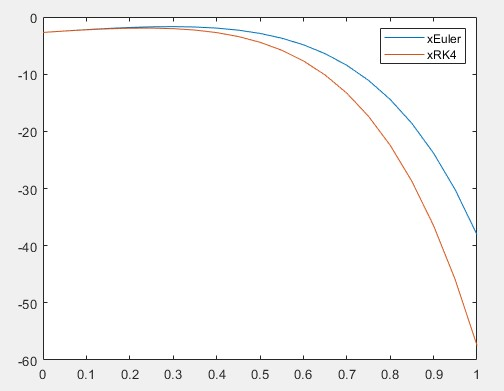
\includegraphics[scale=0.75]{Prim1x.jpg}
			\caption{$x(t)$ iz primera \ref{prim:Euler1}, dobljen z obema metodama}
		\end{figure}
		
		Opazimo, da se rešitvi najprej dobro ujemata, nato pa rešitev, dobljena z Eulerjevo metodo, začne odstopati od te, ki smo jo dobili z metodo Runge-Kutta reda $4$. Na koncu intervala, v točki $1$, je razdalja med rešitvama $19'3764$, kar je seveda nezanemarljivo.
		
		\begin{figure}[H]
			\centering
			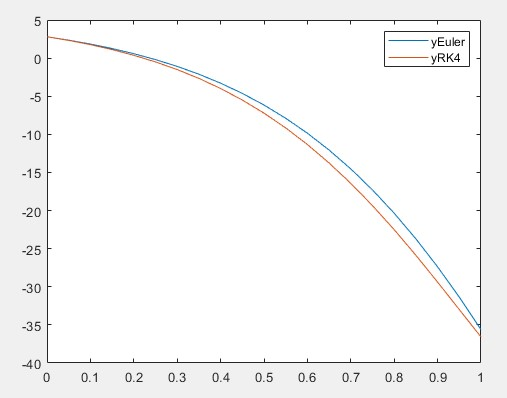
\includegraphics[scale=0.75]{Prim1y.jpg}
			\caption{$y(t)$ iz primera \ref{prim:Euler1}, dobljen z obema metodama}
		\end{figure}
		
		Boljše ujemanje se pojavi v drugi koordinati, kjer se največja razdalja med rešitvama pojavi med krajiščema intervala, v točki $1$ pa je razdalja le $0'9638$. To je še vedno veliko odstopanje, a bistveno manjše od odstopanja v prvi koordinati.
		
		\begin{figure}[H]
			\centering
			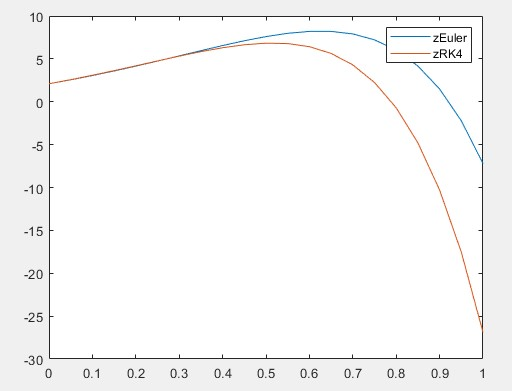
\includegraphics[scale=0.75]{Prim1z.jpg}
			\caption{$z(t)$ iz primera \ref{prim:Euler1}, dobljen z obema metodama}
		\end{figure}
		
		V tretji koordinati se ponovno pojavi opazno veliko odstopanje med rešitvama. Razlika je minimalna v prvi tretini intervala, v krajišču $1$ pa doseže $19'6899$. 
		
		V vsakem primeru zaradi višjega reda konvergence bolj zaupamo rešitvi, dobljeni z metodo Runge-Kutta reda $4$. 
		
		Ker za enačbo iz primera \ref{prim:Euler2} poznamo tudi analitično rešitev, ki se glasi $x(t) = 2\cos(t) + 3\sin(t) + 3t\sin(t)$, bomo grafa numeričnih rešitev primerjali medseboj in z grafom analitične rešitve.
		
		\begin{figure}[H]
			\centering
			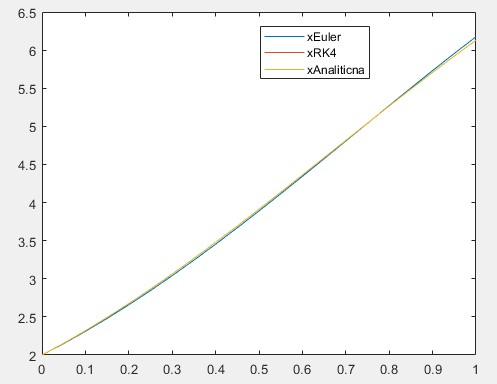
\includegraphics[scale=0.75]{Prim2x.jpg}
			\caption{$x(t)$ iz primera \ref{prim:Euler2}, dobljen z obema metodama in v primerjavi z analitično rešitvijo}
		\end{figure}
		
		Opazimo, da se rešitvi razmeroma dobro ujemata na celotnem intervalu. Še več: Rešitev, ki smo jo dobili z metodo Runge-Kutta reda $4$ se v krajišču od analitične rešitve razlikuje šele na sedmem decimalnem mestu.
		
	
	\begin{thebibliography}{99}
		
		\bibitem{bib:Matlab} J.~Mathews in K.~Fink,~\emph{Numerical methods using Matlab, third edition},~ Prentice Hall, Upper Saddle River, 1999.
		
	\end{thebibliography}
\end{document}